\cleardoublepage
\newrefsection
\chapter{外文翻译}

\section{摘要}

在这篇综述中,我们将讨论了联合反演和约束反演方法的基本原理,并展示了这些方法在文献中应用的几个有启发性的例子。从术语联合反演和约束反演的一些基本定义开始,我使用一个简单的三层模型作为教程,演示了具有不同耦合方法的联合反演的一般属性。特别地,我调查了不同地球物理方法的组合在多大程度上可以限制可接受的模型集,以及在什么情况下结果可能有偏差。关于如何识别这种有偏见的结果以及如何解释负面结果的一些想法总结了教程部分。第二部分的案例研究被选中以突出具体问题,例如选择适当的参数关系来耦合地震和电磁数据,并展示最常用的方法,例如交叉梯度约束和直接参数耦合。在整个讨论过程中,我试图确定未来工作的主题。总的来说,将电磁数据与其他观测相结合似乎已经趋于成熟,并开始从基本的概念验证研究转向回答有关地下结构的问题。通过适用于不同地质情况的多种耦合方法,综合方法可以应用于所有尺度,并有可能为重要的地质问题提供新的答案。

\section{简介}

地球物理观测反演是研究地球地下和了解我们赖以生存的星球的结构和组成的主要工具之一。钻孔通常使我们能够接触到5公里深处的材料,在特殊情况下可达10公里(Huenges等,1997),但只能在特定位置取样。在某些地方,例如金伯利岩管,地质过程将物质从深处输送到地表,并为我们提供来自下地壳和地幔的样本(例如,Griffin等,2009)。然而,我们的大部分知识来自将假设模型计算出的数值模拟的输出与地球表面或附近的地球物理观测结果进行比较。在某些情况下,这些模型是通过正演建模通过反复试验生成的(Leibeckeretal.,2002;Gatzemeier和 Moorkamp,2005;Heise等,2008)。如果这个过程执行得好,我们可以测试关于所调查区域物理结构的不同假设,并深入了解数据对不同结构的敏感性。然而,正演建模通常需要大量试验,因此是一项乏味的任务。此外,模型通常是对地质结构的强烈概括,先入为主的想法可能会影响在此过程中考虑的模型类型。

由于这些原因以及过去几年计算能力的显着提高,如今大多数地球物理模型都是通过正式的反演程序构建的。在这里,我们在数学上定义可接受模型的标准,通常是最终模型预测的数据符合最小二乘意义上的观察结果(例如,Wheelock等,2015),并使用自动算法找到一个或一组满足这些标准的模型。鉴于反演不仅在地球物理学中的重要性,存在大量不同的算法来完成这项任务(Nocedal(2006)、 Snieder和Trampert(1999)、Tarantola(2004)、Menke(2012)、Mosegaard和Hansen(2016))以及大地电磁法(MT)和受控源的特殊情况对地球物理背景下的反演方法进行了很好的介绍Avdeev(2005),Abubakar等的电磁学(CSEM,2009)、Siripunvaraporn(2012)以及Rodi和Mackie(2012)。

尽管有高度精确的算法和深入的研究,地球物理数据的反演实际上总是病态的,即相似的数据可能导致截然不同的模型(例如,Backus和Gilbert,1967)和非唯一的,即无限数量的模型可以解释数据相同程度的不确定性(例如,Munooz和Rath,2006)。这是因为我们只能在地表或地表附近进行测量,并且与地质变化的尺度长度相比,站点之间的距离很大。此外,我们的测量是带限的并且受到噪声的污染(Parker1980,1983)。这导致在解释数据时需要考虑的逆向模型中的歧义。然而,这些歧义的本质是特定于方法的。例如,大地电磁法可以很好地解析电阻层的厚度,但不能解析电阻率,而直流电阻率对其电阻很敏感,即电阻率-厚度乘积(Vozoff和Jupp,1975)。如果我们能够利用这些互补的敏感性,与仅使用单一方法相比,我们有望更好地恢复地球内部结构的形状和特性。

这是联合合作反演的核心思想:我们将来自两种或多种不同类型的地球物理数据集的信息组合在一个反演算法中,目的是改进所得模型。本综述的目的是解释和说明联合反演的不同方法,特别强调电磁方法。我将给出联合反演的工作定义,并将其与其他合并不同数据集的方法进行简要比较和对比。然后我将展示一些精选的使用联合反演方法时展示优势和潜在缺陷的示例。最后,我将尝试总结我们目前所处的位置以及未来的途径。与Haber和HoltzmanGazit(2013)最近对该主题的评论相比,我将重点关注概念和应用,而不是数学细节。

\section{关于联合反演的简介}

出于回顾的目的,我将使用术语联合反演来表示在单个计算算法中使用单个目标函数对不同类型的数据进行反演并且在整个反演过程中同时调整所有模型参数的所有方法(Moorkamp等,2016b)。特别感兴趣的是联合反演方法,它结合了不同的物理特性,例如电导率和地震速度,因为这些提供了巨大的潜在好处,但也带来了特殊的问题。相比之下,合作反演包括仅对单个数据集进行反演并将另一个反演的结果用作参考的方法(如,Paasche和Tronicke,2007)。在这篇评论中,我不会讨论反演后积分背后的理论,其中以定量方式检查从独立反演中检索到的模型的关系(如,Bedrosian等,2007),并且可以在Paasche中找到很好的概述(2016)、Bedrosian(2007)和Hansen等(2016)。

正如联合反演的定义所暗示的那样,首要和关键步骤之一是定义优化算法将最小化的目标函数。在最一般的形式中,这个目标函数可以写成以下形式:
\begin{equation}
    \Phi_{joint}(\mathbf{m}) = \Phi_{data}(\mathbf{m}) +\lambda \Phi_{reg}(\mathbf{m})+\mu \Phi_{coupling}(\mathbf{m})
\end{equation}

这里$\Phi_{data}(\mathbf{m})$和$\Phi_{reg}(\mathbf{m})$在数学上定义了模型参数的不同子集之间的关系。注意在这种通用表示法中,模型向量$\mathbf{m}$可能包含与非 常不同的数量相关联的元素。例如,当联合反演分层地球结构的大地电磁和地震走时数据时,前N 个模型参数 可以是反演中使用的N个层的电阻率,第二个N个模型参数指定相同层的地震速度。耦合项然后在这两组模 型参数之间建立关系,该关系指定我们要执行哪种联合反演。

对于协同反演,数学公式看起来是一样的。同样,我们有一个数据误差项、一个正则化项和一个耦合项,只是 现在数据误差和正则化仅针对电阻率进行计算,例如,地震速度模型被认为是固定的并且仅用于耦合项以最大化模型之间的相似性。下图显示了两种方法之间的差异,作为反演的流程图。

我现在将讨论一系列非常简单的实验,以说明联合和协作反演的一些基本性质以及常见的耦合方法及其性 质。所有实验的基础是从一个简单的一维三层模型计算的数据(图\ref{trans2})。为了进一步简化讨论并提供帮助可视化,我也假设知道最上层和最下层的物理特性(电阻率和地震速度)和厚度,并且只寻求中间 层的厚度和物理特性。因此,逆向问题简化为为每个地球物理数据集寻找两个模型参数,例如MT 的第二层电阻率和厚度,并且很容易将可能解的范围绘制为简单的散点图。

\begin{figure}
    \centering
    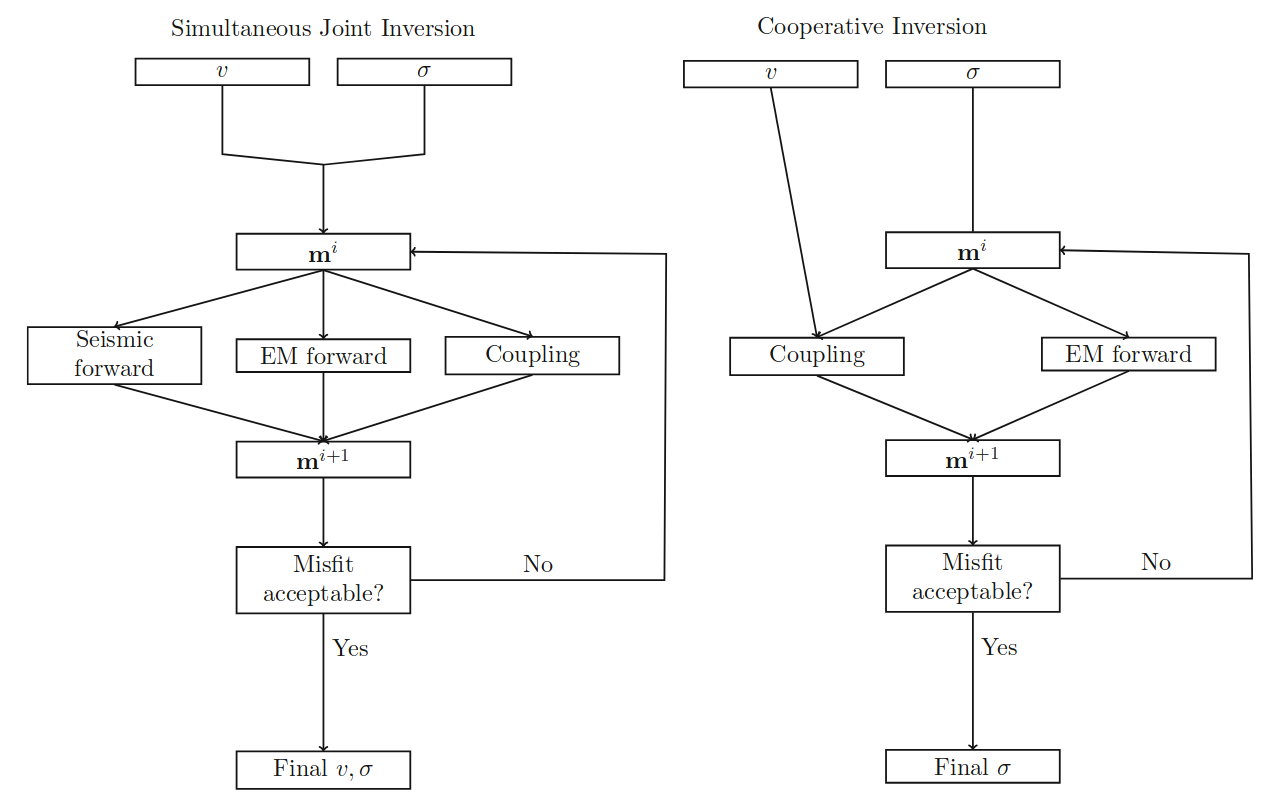
\includegraphics[width=0.9\textwidth]{trans/trans_1.png}
    \caption[]{联合反演算法(左)和协同反演算法(右)的简化流程图(Moorkamp等, 2016 b)。两种方法之间的主要区 别在于,对于协同反演,进入耦合约束的一个量(此处地震速度 v)在整个反演过程中不会发生变化,而所有量都在联合反演中进行调整} \label{trans1}
\end{figure}

\begin{figure}
    \centering
    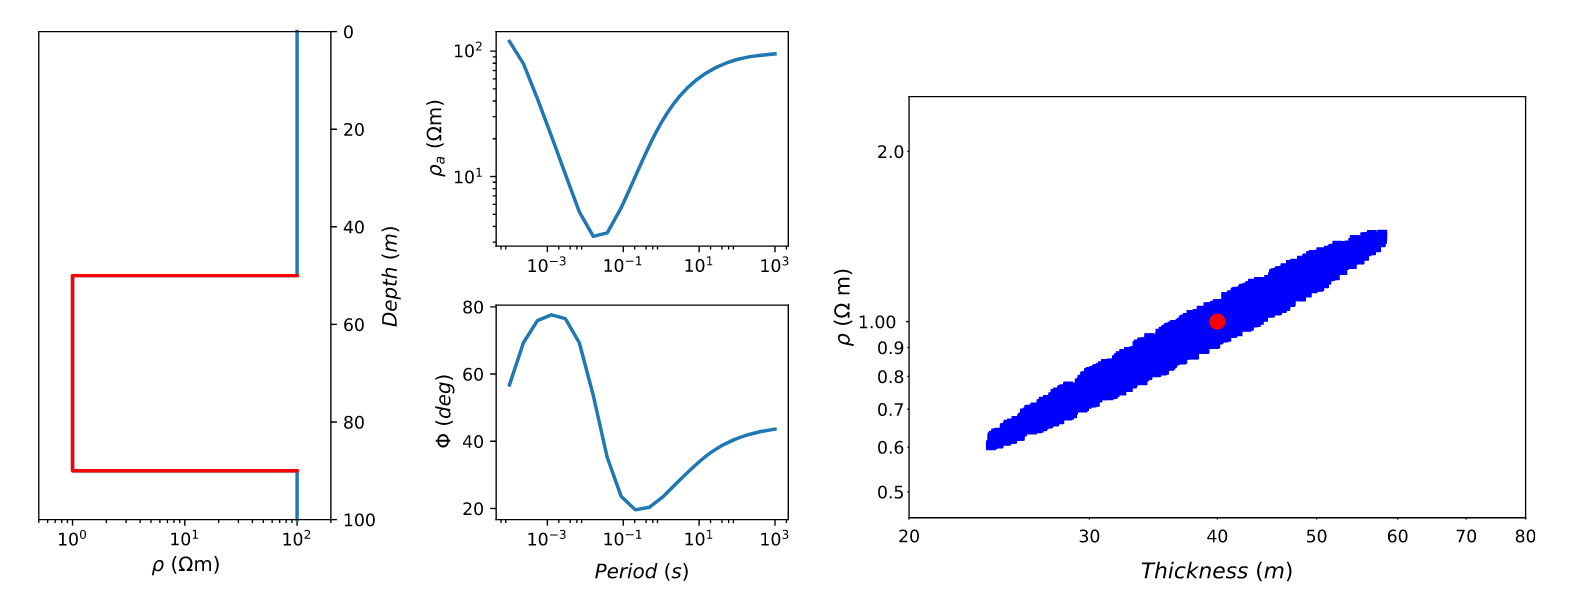
\includegraphics[width=0.9\textwidth]{trans/trans_2.png}
    \caption[]{简单的大地电磁测试模型(左),该模型的正向响应(中)和仅反演 MT 数据时可接受的反演模型空间(右)。在整个教程 中,仅假设最上层和最下层是已知的,只求中间层(标记为红色)的厚度和电阻率} \label{trans2}
\end{figure}

图\ref{trans2}显示了真实模型(左),其中我们要反演的层标记为红色。从模型(中间的图)预测的大地电磁数 据显示典型的三层响应。为了说明可行的解决方案,我简单地生成了大量试验电阻率和厚度的随机组合,计算出与真实响应的误差,并保留拟合数据的实部和虚部均在 2\%以内的参数组合。生成的可行解在图\ref{trans2}中显示为蓝点,真实值显示为红色。这个简单的实验证明了众所周知的无法恢复薄导电层的电阻率和厚度,而不是层电导,即电导率与厚度乘积受到很好的约束。该特征在反演问题的解集中清晰可见。查看反演问题的解,该层可以具有20 m和60 m之间的任何厚度,同时也有合适的电阻率。

\begin{figure}[H]
    \centering
    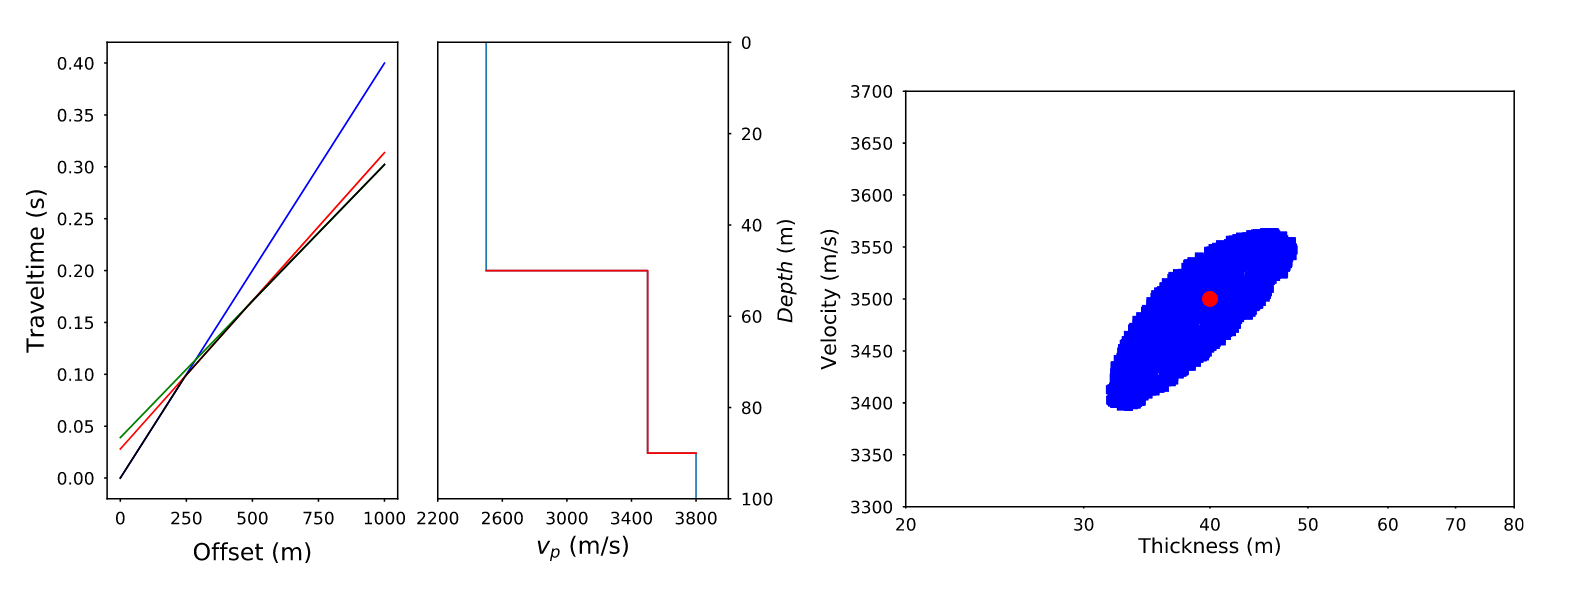
\includegraphics[width=0.9\textwidth]{trans/trans_3.png}
    \caption[]{单独反演走时时的地震数据(左)、真实模型(中)和一组可接受的速度与厚度的组合(右)。对于图3.2中的 MT情况,只有 中间层(标记为红色)的属性是未知的} \label{trans3}
\end{figure}

如果我们在同一位置进行地震折射实验并仅从这些测量中确定一组反演的解,我们将得到图\ref{trans3} 所示的 结果。在这种情况下,地震折射数据也显示出模糊性以及速度和速度的范围解释假设误差内观察结果的厚度值。 然而,与大地电磁方法相比,可能的厚度值范围更窄,在30到 45m 之间。联合反演的核心思想是在两种方法感知相同结构的假设下,找到解释两个数据集的模型将导致更好地恢复这些 结构。现在,我将讨论最常用的假设,并通过这些简单的示例演示如何使用它们、可以期待什么样的改进以及存在 哪些缺陷。


\subsection{结构耦合}

关于不同地球物理方法之间的关系,我们可以做出的最普遍的假设之一是它们感知地球内部的相同地质结构,特 别是它们的边界。因此,如果有任何速度或电阻率异常,它们应该发生在同一位置。因此,结构联合反演方法不规定 不同物理参数之间的任何直接相关性,而是使用这些参数变化之间的空间关系来耦合不同的方法(Haber 和 Oldenburg,1997; Gallardo 和 Meju,2003)。我将在下面的案例研究中讨论联合反演中常用的不同结构 关系的一些例子。对于分层地球模型,一个简单的结构关系是假设所有方法的反演中的层边界都处于相同深度(如, Manglik 和Verma,1998; Moorkamp等,2007;泽瓦洛斯等,2009; Moorkamp 等,2010; Roux 等,2011; Juhojuntti 和Kamm,2015)。图\ref{trans4}显示了假设边界重合时我们的简单示例的两个数据集的可接受模型范围。

\begin{figure}
    \centering
    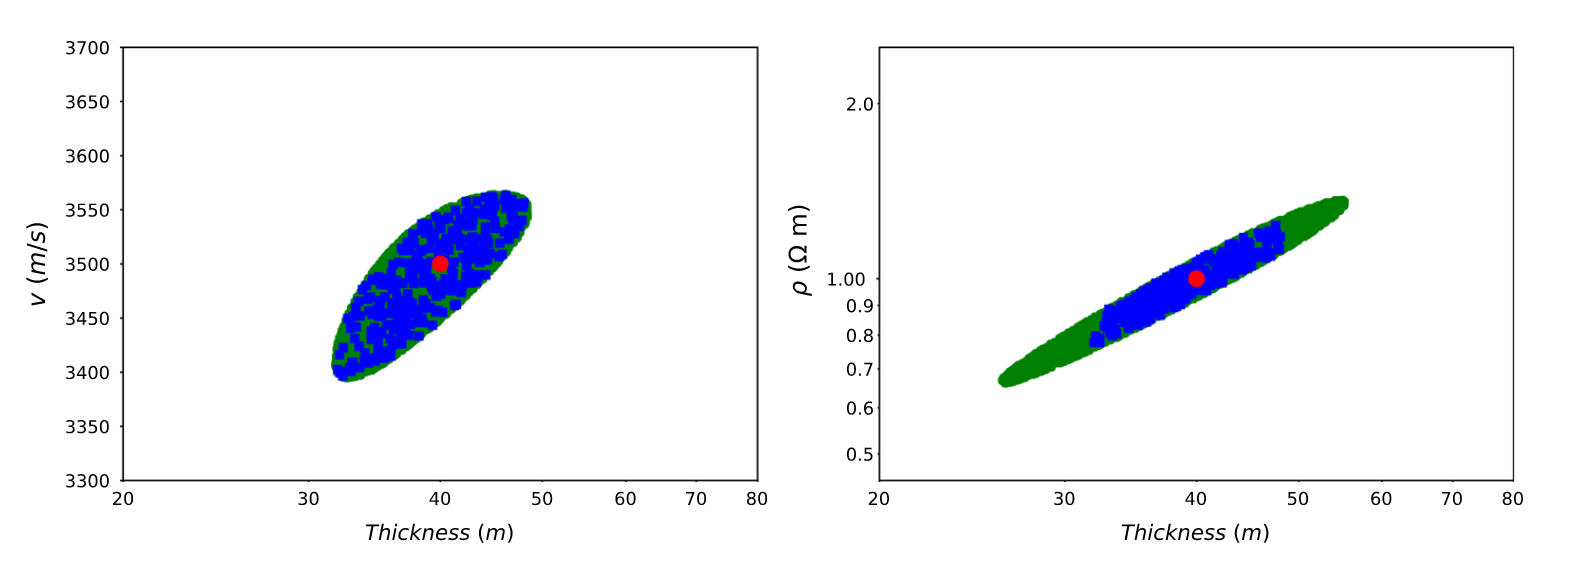
\includegraphics[width=0.9\textwidth]{trans/trans_4.png}
    \setcounter{figure}{3}
    \caption{一组可接受的速度-厚度(左)和电阻率-厚度(右)组合,用于单独反演和联合反演,具有基于重合层厚度的结构约束。单 独反演的可接受模型标记为绿色,而联合反演模型标记为蓝色}\label{trans4}

\end{figure}

由于没有采用电阻率和速度之间的关系,因此这种方法主要限制了允许的层厚度范围。鉴于大地电磁数据的这个范围较大,允许的电阻率模型的范围减小,而可接受的地震模型的范围与单独的分析相同。总的来说,结构耦 合实现了联合反演的主要目标,以减少可接受模型的范围,即使在这种情况下仅针对一个参数子集。显然,对于更为实际的反演,即假设地球是分层的,情况也会更加复杂。当同时反演所有三层的属性时,不同层的厚度和物理参 数之间存在显着的相互作用。例如,大地电磁数据对顶层厚度具有合理的敏感性,该信息将有助于约束地震模型, 进而有助于约束第二层的厚度。因此,在现实世界的联合反演中,并不总是那么清楚哪种方法主导分辨率属性,并 且在许多情况下,不同的方法驱动模型域不同部分的反演(Jegen 等,2009 ; Heincke 等,2009、2014; Demirci 等, 2017 )。我将在应用部分讨论其中的一些问题;现在我将继续这个简单的 例子,因为它提取了联合反演的许多重要方面。

进一步考虑层厚度的分辨率如何从速度模型转移到电阻率模型,以及它如何影响图\ref{trans4}中可接受模型的范围,同 样清楚的是,我们将找到适合两个数据集的模型,即使厚度真实速度模型中的层数不同于真实电阻率模型。60 m的厚度在大地电磁数据的可接受范围内,因此,将层厚度为 40 m的电导率模型与地震厚度为60 m的组合将 产生一个联合模型,该模型在假设的范围内拟合两个数据集噪音水平。在最极端的情况下,真实地震模型的层厚 可能超出大地电磁数据的允许范围,但考虑到地震结果的不确定性,这两个区域重叠,我们找到了一个适合两个数据集的联合模型到可接受的水平,但两种方法都处于极端不确定的状态。

在这个非常简单的例子中,进行协同反演最直接的方法是选择一个适合地震数据的模型并将其用作参考MT的模型。在最受约束的情况下,我们可以将该模型的层厚度作为真实层厚度的估计值,并且只搜索电阻率。结果 是一组非常有限的可接受模型。然而,如果估计厚度与真实厚度不同,则真实模型将不包括在可接受的模型集中并 且估计的电阻率将有偏差。一种更接近当前实践的方法(Kalscheuer等, 2015)是在目标函数中包 含一项,要求层的厚度尽可能接近地震估计值。

\begin{figure}[H]
    \centering
    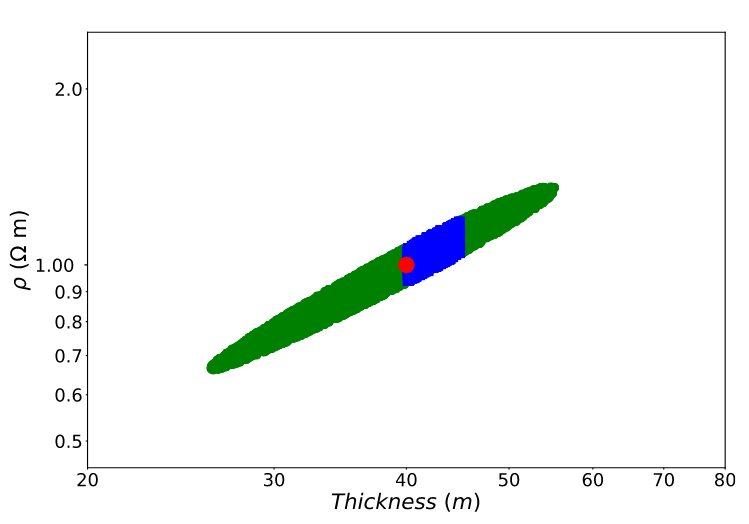
\includegraphics[width=0.9\textwidth]{trans/trans_5.png}
    \caption{无约束反演(绿 色)和层厚度被约束匹配的反演的一 组可接受的电阻率-厚度组合 941 5m 以内的推断地震边界。在此示 例中,真实模型是可以接受的解集中的一 部分;然而,如果我们在地震数据允许的范围的最末端选择了一个参考模型, 它可能不是一组真实的模型}\label{trans5}

\end{figure}

图\ref{trans5}显示了可接受的模型,这些模型与 50 m 的估计层厚度一致,误差在 10\%以内。与指定固定层厚相比,可接受 模型的范围有所增加,但仍小于结构耦合联合反演。根据厚度估计和我们在估计中指定的不确定性,真实模型将 是否包含在可接受的模型中。在我们有关于可接受地震模型范围的全部信息的情况下,例如,从概率反演方法,结 果将与联合反演结果相同。然而,如果我们只有一个模型和模型不确定性的临时估计,那么结果在很大程度上取决于这两者与真实模型的关 系。 MT的模型。在最受约束的情况下,我们可以将该模型的层厚度作为真实层厚度的估计值,并且只搜索电阻率。结果 是一组非常有限的可接受模型。然而,如果估计厚度与真实厚度不同,则真实模型将不包括在可接受的模型集中并 且估计的电阻率将有偏差。一种更接近当前实践的方法(如Kalscheuer等, 2015 )是在目标函数中包 含一项,要求层的厚度尽可能接近地震估计值。 起初,看到合作或约束反演比完全联合反演更能限制可接受模型集可能会令人惊讶。虽然解释相对简单:由于 无法对参考模型进行调整,除非我们考虑完整的后验模型协方差,否则地震数据的不确定性已从等式中剔除。因 此,必须特别小心地检查作为此类约束反演结果的模型,并且可以将其视为假设检验的特殊情况,如下所述,即我 们已经证明存在类似于地震参考模型并适合大地电磁法的模型数据。

\subsection{基于参数关系耦合}

通过结构耦合方法不对不同地球物理方法之间的关系做出强假设,因此具有广泛的适用性。正如示例所示,与单独的反 演相比,这样做的结果可以适度提高分辨率。如果我们在反演中利用更多关于地球的信息,我们可能会显着改善 我们的结果。这通常适用于所有逆向方法,额外的先验信息限制了可接受模型的空间,但存在使解决方案产生偏差 的风险(Tarantola,2004; Mosegaard和 Hansen,2016)。指定速度和电阻率之间的关系是引入此类信息的一种方式,并且将反演的地震折射和大地电磁部分紧密联系起来。

让我们假设从一些钻孔数据或其他信息来源我们对第二层有以下估计形式的关系\ref{eq1}:
\begin{equation}
    \log \rho = \frac{v}{3500} \label{eq1}
\end{equation}

\begin{figure}[]
    \centering
    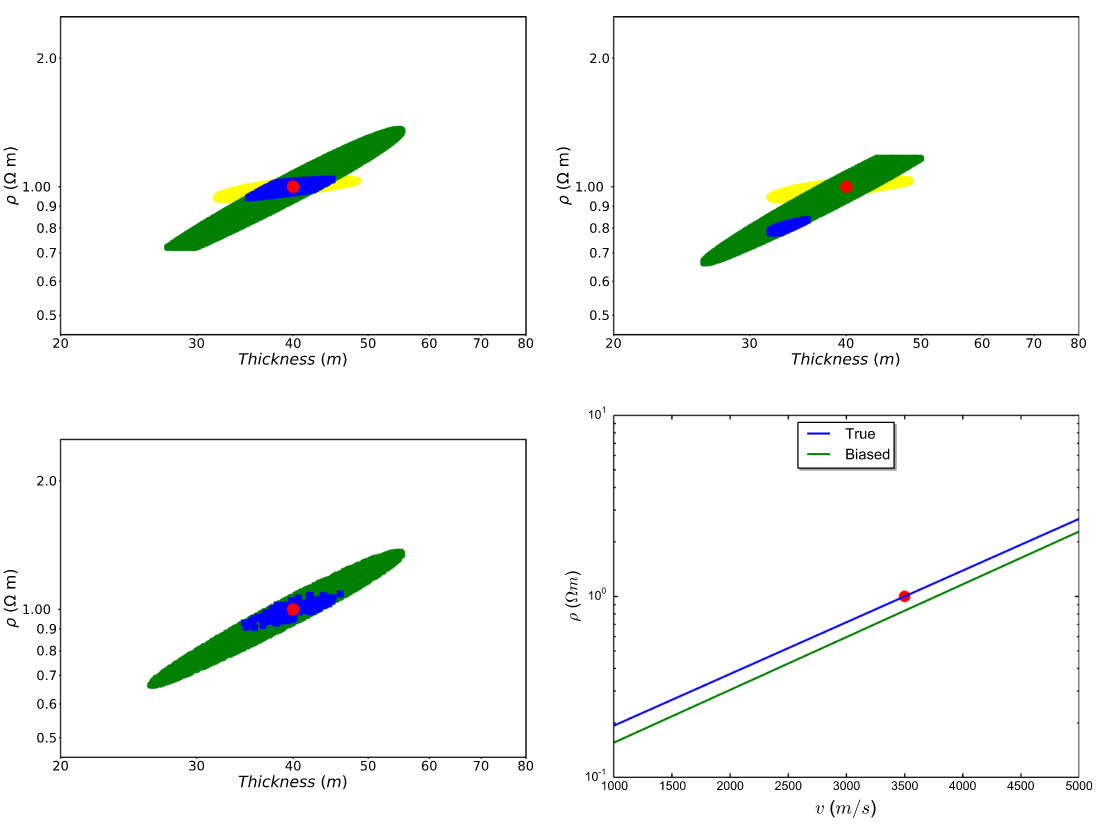
\includegraphics[width=0.9\textwidth]{trans/trans_6.png}
    \setcounter{figure}{5}
    \caption{具有参数关系的联合反演可接受的电阻率-厚度组合。当关系被认为是准确的并且假设的参数关系与真实关系匹配时(左 上角),我展示了解决方案。和以前一样,单独反演的可接受模型显示为绿色,而联合反演模型显示为蓝色。此外,通过关系投影 到电阻率-厚度的地震模型以黄色显示。我还展示了假设关系存在偏差(右上角)以及关系不被视为精确但作为约束包含在内 (左下角)时的结果}\label{trans6}

\end{figure}

对于其他层,这种关系是不合适的,但在我们的简单示例中,假设这些层的参数是已知的。此外,在文献中有一 些例子,其中参数关系仅假定在特定深度范围内有效(如,Hoversten 等,2006;Chen等,2007 )。如果我们假设这个关系是精确的并且没有任何错误,我们可以用它来规定关于地震速度的大地电磁学和地震学的反演问题,并使用\ref{eq1}进行速度和电阻率之间的转换。这提供了两种方法之间的强耦合,因为层中速度的变化对大地电磁阻抗的误差有直接影响。\ref{trans6}显示了针对这种情况的电阻率和厚度方面的可行解决方案。我们可以看到,在正确的参数关系下,可行解的解空间受到限制,因为不同解之间的交集是很小的。这证明了这种高度耦合的联合反演方法的力量和潜在的重要信息增益。


具有直接参数关系的联合反演的一个特例是所谓的岩石学/岩石物理联合反演方法。那里的关系不是根据 一个地球物理参数作为另一个函数来表达的,而是所有地球物理量(例如,电阻率、速度、密度)都是孔隙度和 渗透率等量的函数(如,Chen等,2007 ;Gao 等,2012;Commer 等,2014 )或温度和地 幔成分(例如 Afonso等,2016 ;Zunino 等,2016 )。从概念上讲,这些方法与具有相同注意事项的 地球物理量之间的直接耦合相同,但是,它还有一个额外的优点,反演结果与地质研究的质量息息相关。

在实践中,我们很少能够高精度地确定经验参数关系。例如,钻孔测井数据显示出明显的分散性,尚不清楚 厘米尺度的测量是否可以用于数十至数百米甚至千米尺度的反演问题(Moorkampet al.2013; Panzner et al.2013)。 2014)。图6演示了假设参数关系不正确时会发生什么。这里我用了

\begin{equation}
    \log \rho=\frac{v}{3428}-1.1
\end{equation}

在反演中而不是上面的正确方程。对于这种轻微扭曲的关系,仍然可以找到可行的解决方案,但这些与真实值 相比存在偏差。此外,可行模型的小区域暗示了一个高度精确的答案,但真正的模型不包含在该解决方案空间 内。因此,必须特别小心地研究这种强耦合联合反演方法的结果。

合并参数关系但降低偏差风险的一种方法是将关系作为约束包括在内,而不是使用它直接在参数之间进行 转换。在这种情况下,我们在电阻率和速度方面保持反演的参数化,但除了拟合数据之外,还要求模型参数在最 小二乘意义上接近假定的参数关系。这是方程式中耦合项的第一个例子。到目前为止,这仅隐含在公共层厚 度或简化为单一物理特性中。约束可以是函数的形式(如Heincke等,2014 ;Kamm等, 2015 ),也可以是关系值应归入的聚类中心(Carter-McAuslan等,2015 ;Sun 和 Li,2016 )。

\ref{trans6}显示了使用基于方程式的约束运行反演的结果。而不是假设方程式中所示的正确值的固定参数关 系。 正如预期的那样,允许模型的范围增加了,因为模型的电阻率-速度组合不再必须完全位于假设的关系 上,而是散布在它周围。因此,在对关系的整体形状有信心但个别值可能分散在总体趋势周围的情况下,基于约 束的联合反演可以允许偏离该趋势。如果约束基于不正确的关系,则简单示例(未显示)的可接受模型范围与为直接关系显示的模型范围非常相 似。同样,允许模型的范围是有偏差的,不包括真实模型。在基于最小化方程式中所示的加权和的实际反演中,拟合数据和满足关系会相互权衡,类似于正则化和数据失配权衡的方式。可以使用这个权衡以识别参数关系的问题,接下来我将讨论识别此类问题的一般策略。

\subsection{识别问题和检验假设}

上述例子突出了使用地球物理数据联合反演时的潜在的陷阱。在进行联合反演时,我们通过假设重合结构或参数关 系引入额外的先验信息。如果此先验信息不正确,可能会导致有偏差的结果。在前面的示例中,我总是绘制适合低 于假定误差水平的数据的可行解的空间,以说明解的分布。然而,并非所有这些解决方案都同样适合数据。在这种 情况下,输入数据没有噪声,一些解决方案完全符合数据,而其他解决方案则刚好符合假设的噪声水平。对于具有 可靠误差信息的真实数据,目标失配应该是RMS 为1,即平均而言,观测值在估计误差内拟合。然而在实践中,真 实数据很少能符合该水平(如Rao 等,2014;Peacock 等,2015;Yang 等,2015)。这可能 有多种原因,包括过于乐观的错误估计或无法在反演中包含足够小的表面结构。因此,在进行任何联合反演之前, 必须对每个数据集进行单独反演,以确定每个数据集的参考误差(如Linde等,2006;Moorkamp 等,2013 )。执行这些单独的反演还有助于找到合适的正则化参数(如Hansen1992),这些参数可 以针对联合反演进行缩放(Moorkamp等,2016a)。

如果具有可比模型离散化的联合反演未能将数据拟合到与单独反演相同的失配水平,则可能是因为方法之间 的耦合引入了非线性部分(Lelie`vre和Farquharson 2016;Heincke等,2016)。2017)或者因为选择 的耦合约束不合适(Moorkamp等,2007)。可以通过改变联合反演的起始模型来识别非线性,例如从最合适 的个体反演结果而不是半空间或类似模型开始。当从拟合良好的模型开始时,联合反演应该增加耦合约束下不同 模型之间的相似性,最终模型应该与各个模型具有可比的失配。如果达不到,说明耦合约束不合适,即反演中对地 球的假设不正确。

精心构造的耦合约束(例如,基于假设的岩石物理模型的参数关系)不适用于特定数据集的联合反演的结果 最初可能令人失望。然而,如果我们能够证明我们可以排除其他因素,例如上面讨论的非线性、参数化问题或数据 错误,那将是一个非常强大的结果。传统上,不同方法之间的耦合被认为是已知的先验信息,联合反演的重点是使 用这些附加信息来改进与单独反演相比的结果。然而,另一种看待它的方法是,通过执行联合反演,我们检验了模 型存在符合所选耦合方法的假设,并同时解释了观察结果。当联合反演失败时,由于我们无法将数据拟合到令人 满意的水平,我们证伪了这一假设并证明了耦合约束不能反映地质情况。当然,存在大量可以通过这种方式证伪 的可能的耦合约束,其中大部分是无意义的。相反,如果有可能通过仔细的分析表明地幔电阻率和速度的变化不 能简单地用成分的简单变化来解释,例如,我们就已经了解了一些关于地球的有价值的东西。

对于典型的地球物理反演问题,通常不存在拒绝反演结果的明确标准。尽管大多数逆向算法的核心最小二乘 拟合是基于可靠且发达的数学基础,但经常违反基本假设,例如误差的高斯分布(Matsuno 等,2014)。除了如 上所述使用单独反演的失配作为基准之外,分析联合反演结果的另一种有用方法是查看不同数据集的拟合和满 足约束如何相互作用。

图7显示了参数关系的失配与地震数据的失配,所有模型都在可接受的水平上拟合两个数据集。当反演中假设 的关系正确时(左图),具有低地震失配的模型也比具有较大地震失配的模型更好地匹配约束。相比之下,当假 设的参数关系不正确时(右图),不存在既具有低地震失配又与约束良好一致的模型。因此,绘制不同数据集和 约束的不匹配组合可以揭示它们是否相互兼容或最小化一个以恶化另一个的匹配为代价。在实际反演中,可以通 过改变目标函数不同项的权重(Thompson 等,2016)或使用专门设计的多目标最小化算法(Kozlovskaya等, 2007;Moorkamp 等, 2007)来构建此类图的应用程序, 2010; Roux 等,2011; Schnaidt 和 Heinson2015; Lelie`vre等,2016;Niri和Lumley,2016 )。

\begin{figure}[H]
    \centering
    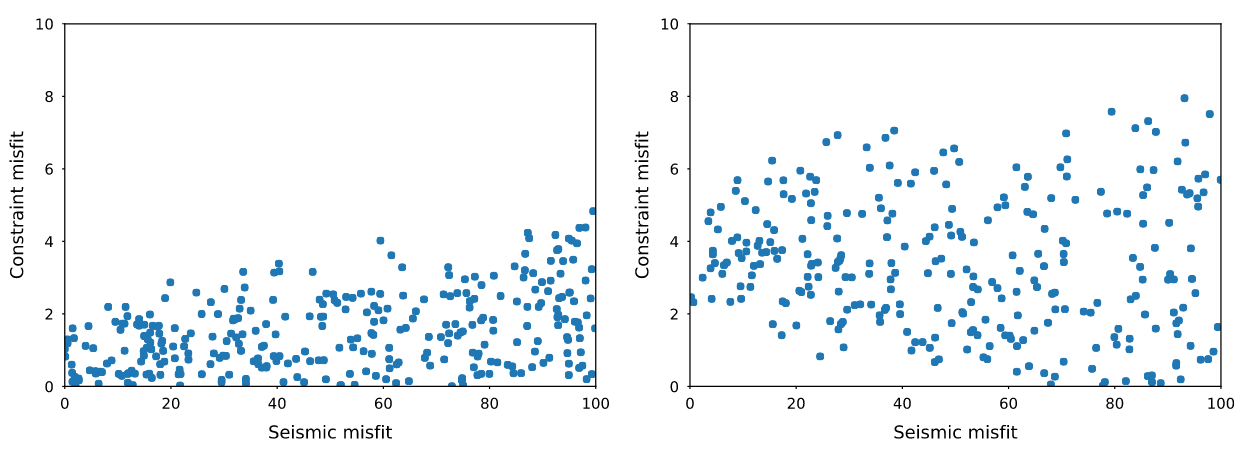
\includegraphics[width=0.9\textwidth]{trans/trans_7.png}
    \setcounter{figure}{6}
    \caption{为正确假设的参数关系(左)和有偏差的关系(右)拟合地震数据和匹配参数关系约束之间的权衡。可以清楚的看到当关 系不正确时,不存在同时满足数据和约束的模型} \label{trans7}

\end{figure}

在整个前面的讨论中,我一直专注于电磁和地震数据,因为与单独反演相比,这种方法组合有望带来显着改进, 并且需要在反演中耦合不同的物理量。当然,该讨论也适用于组合电磁数据和重力数据(如,Maier等, 2009),但在一定程度上,即使将不同类型的电磁数据一起反演也是如此(Commer和Newman, 2009 ; Newman等, 2010;Haroon 等,2015)或具有直流电阻率数据的电磁(如, Candansayar和Tezkan2008; Yogeshwar 等,2012; Hoversten 等,2016)。即使在后一种情况下,所 考虑的物理参数是电导率,大地电磁法对水平电导率敏感,而受控源方法对水平和垂直电导率敏感,这会导致精 细层状沉积环境中的有效各向异性(Newman 等, 2010)).因此,通过不同方法反演的电导率将不同, 并且必须在联合反演中引入适当的耦合方法,例如,通过在反演中引入电各向异性(Commer和Newman2009),数据失配将与反演允许的各向异性量进行权衡。

\section{实践中一些集成分析的例子}

前面的简单示例说明了联合反演的概念,现在我将讨论这些概念在实际数据中的具体应用。综合方法现已应用于 广泛的领域,最近发表的评论涉及水文地球物理学(Linde和Doetsch 2016)、矿物勘探(Lelie`vre 和 Farquharson,2016 )、油气勘探(Moorkamp等,2016b)的联合反演、岩石圈成像(Afonso 等, 2016)和深部地幔研究(Zunino等,2016)。在这里,我将重点介绍这些评论未完全涵盖的一些最新 工作和方面。

\subsection{直接参数耦合联合反演}

作为第一个案例研究,我将比较 Panzner 等(2016)与 Heincke等(2017)的结果。
这两项研究调查了同一地区并使用了相似的数据集。然而,关于如何组合数据集的方法和几种选择是不 同的。因此,这种比较是展示主观选择在实践中如何导致不同结果的好方法。这两项研究的目标是对法罗群岛东 南部沿所谓的 Flare\ 6 线的亚玄武岩沉积物进行成像。玄武岩的厚度和下方沉积物的几何形状对油气勘探具有 重要意义(Christie 和 White, 2008;Manglik等,2009;Patro等,2015),因为它决 定了油气藏的潜在前景。 这两项研究都使用地震走时和电磁数据的组合作为反演方法。然而,虽然Panzner等(2016)使用MT 和海洋可控源电磁数据 (CSEM) 的组合,Heincke 等(2017)仅利用大地电磁测量,但在反演中也包括重力 数据。此外,Panzner 等(2016)使用不同数据集的顺序分析,其中单独执行反演,但信息在单独的反演之间交换。 这些类型的集成工作流程通常用于油气勘探而不是全联合反演,因为全联合反演被认为是棘手的(Um等, 2014),或者因为反演的主要目标是生成改进的迁移模型地震反射数据(Colombo和Stefano 2007; Colombo等,2008; De Stefano等,2011;Colombo 等,2014; Cui等,2015;Takam Takougang 等,2015)或全波形反演(Zerilli等,2016 )、海因克等(2017),相比之下,对所有三 个数据集进行完全联合反演。

\begin{figure}[]
    \centering
    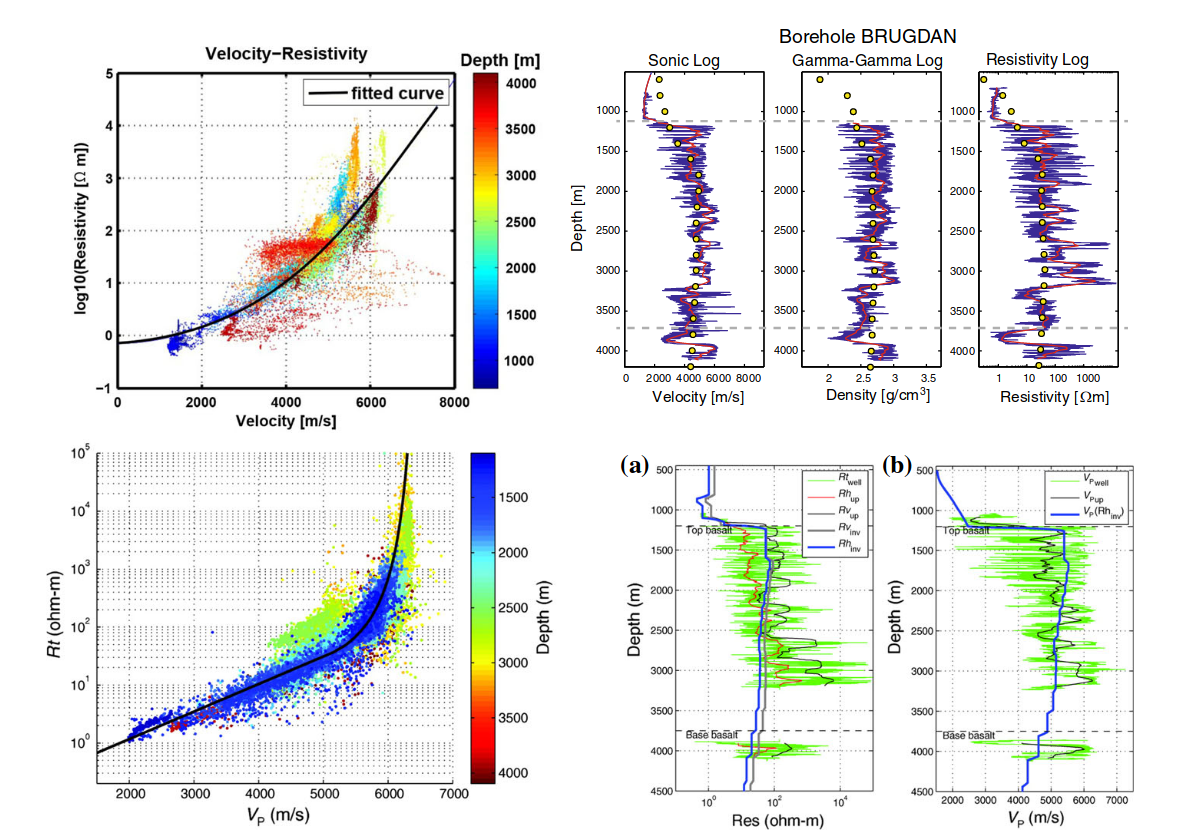
\includegraphics[width=0.7\textwidth]{trans/trans_8.png}
    \caption{Heincke 等研究中使用的 BRUGDAN钻孔(右上)测井数据的速度-电阻率(左上)交会图和深度图。 (2017)。下面一 行显示的信息与 Panzner等使用的信息相同(2014)}

\end{figure}

\begin{figure}[]
    \centering
    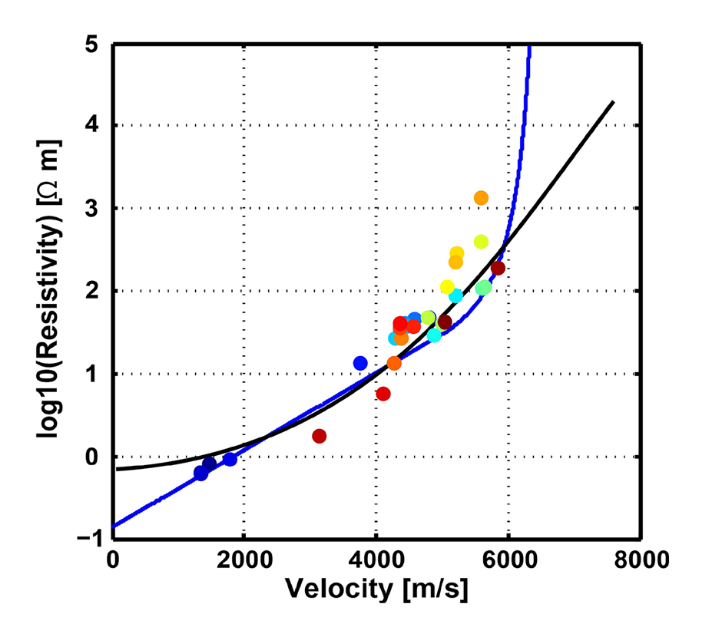
\includegraphics[width=0.5\textwidth]{trans/trans_9.png}
    \caption{平均为 BRUGDAN钻孔的测井数 据的速度-电阻率交会图。间隔为100m。每个点的颜色对应于海 底以下的深度,Heincke 等估计 的速度-电阻率交叉关系。(2017)(黑线) 和 Panzner 等使用的速度-电阻率 关系(2014) }

\end{figure}

就不同方法之间的耦合而言,两项研究都采用了非常相似的方法,并利用该地区钻孔的交叉属性关系来关联 地震速度和电阻率。图8显示了交叉特性图和拟合关系。从这些图中可以清楚地看出,这两种关系只是地下参数真 实变化的近似表示。

速度和电阻率都显着分散在该关系预测的值周围。这部分是由于钻孔测量中的噪声,但也是由于岩性的细微尺度 变化。因此,当平均到 100 m 的尺度时,考虑到个体网格的数量,散射不那么明显,并且这种关系相对是合适的。

尽管如此,基于相同的观测数据,两项研究都选择了不同的参数化来表示参数关系。对于小于 6000 m/s 的 P波速度,差异相对微妙,而对于更高的速度,Panzner等(2016)的关系预测的电阻率明显高于 Heincke 等(2017)的关系。

尽管乍一看差异可能看起来很显着,对于大于6200m/s的速度,预测电阻率存在一个数量级或更多的 差异,但实际上对反演结果的影响并不那么强烈。首先,只有在非常薄的地层中才能达到如此高的速度,并且大部 分钻孔中的平均速度在 4000 和 6000m/s之间变化,这两种关系非常相似。其次,这些高速和高电阻率发生在被 导电沉积物覆盖的玄武岩中。大地电磁数据仅解析了此类结构的最小电阻率(Chave和 Jones,2012),而最大 电阻率不受约束。因此,MT 数据允许任何高于某个阈值的电阻率值,但正则化将限制电阻率。两项研究的反演结 果都证实了这一点。在这两种情况下,恢复的电阻率都不超过 100 Xm。

尽管在这种情况下参数化的差异似乎对反演结果没有显着影响,但这种比较突出了寻找跨属性关系的适当表 示的困难以及联合反演方法的用户仔细考虑他们的要求选择。很明显,在许多情况下,通过连续数学函数的简单近 似是不合适的。聚类方法(Paasche 和 Tronicke,2007;Paasche等, 2010; Sun 和Li,2016 , 2017)为某些场景提供了一种替代方法,但也涉及用户的多种选择,并假设岩性可以用有限数量的聚类中 心。因此,寻找跨属性关系的可靠表示并评估其在一系列条件下的可靠性是联合反演和综合分析中最紧迫的任务 之一,在我看来,这是一个有待进一步研究的富有成果的领域。

图10显示了两项研究的反演结果,其中Brugdan 钻孔(Schuler et al. 2012)在两个图中进行了比较。两种 模型的玄武岩层的整体几何形状和厚度相似,但在一些细节上存在差异。特别是,Panzner 等的模型(2016)预测与Heincke 等的模型相比,钻孔附近玄武岩厚度的变化明显更强,并显示了可能与预裂谷基底 相关的更深的高速结构,这些结构没有出现在 Heincke 等的模型中(2017)考虑到不同数据集的敏感性 (Panzner等,2016 年的图 10),添加 CSEM数据有助于解析这些结构。相比之下,(Heinckeet al. 2017)包含的重力数据似乎对解析深度结构贡献不大。

\begin{figure}[H]
    \centering
    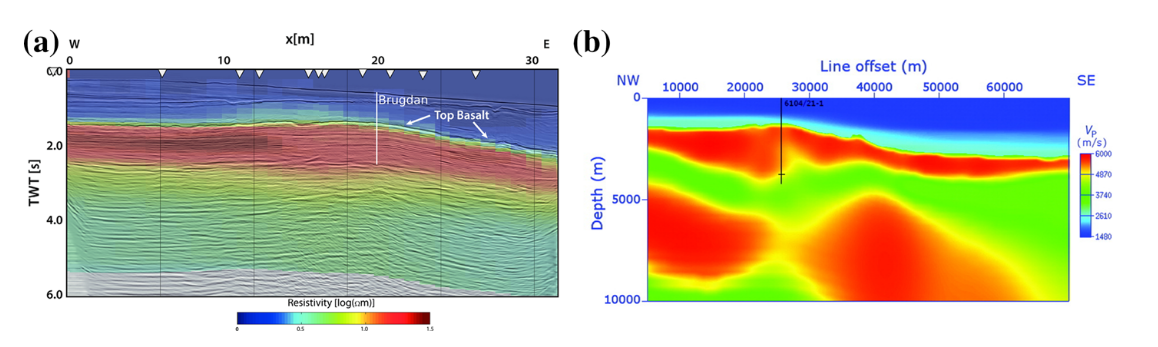
\includegraphics[width=0.9\textwidth]{trans/trans_10.png}
    \caption{Heincke 等的联合反演模型(2017) (左)和 Panzner 等(2014)(右)。}

\end{figure}

\subsection{具有结构约束的联合反演}

第二个例子取自Gallardo 等(2012)也与油气勘探有关。随着新资源勘探进入地质复杂的地区,整合不同类 型数据的价值已被业界认可,并已进行大量投资以开发整合平台(如,DellAversana等, 2016)和赞 助案例研究为了获得必要的经验(如,Colombo等,2010;Chen 和 Hoversten,2012 ; Moorkamp 等,2011; Roberts等,2016)。此外,在过去十五年中,所谓的非地震技术在勘探工作流程中的重要性有所增加(如Constable, 2010; MacGregor和Tomlinson,2014; Strack,2014;Streich,2016)。在这种情况下,研究的重点是巴 西近海的桑托斯盆地,在何种程度上整合地震、大地电磁、重力和磁力数据有助于约束盐和碳酸盐单元的几何形 状。由于结构的陡峭侧翼和地震能量的内部散射,盐结构尤其难以用传统的地震反射方法成像(如Key 等, 2006; Hokstad 等, 2011 )。鉴于桑托斯盆地具有高度可变物理特性的不同岩性的范围,很难构建岩石特性关系,并且很可能任何构建的 关系在研究区域的重要部分都无效。因此,Gallardo 等 ,2012)使用交叉梯度(Gallardo和 Meju,2004、 2007、2011 ;Meju和Gallardo,2016),这是一种多功能的结构约束,已成为联合反演中最流行的耦合方法之 一(如,Linde等,2008; Doetsch等)根据场景的不同,这些耦合方法在某些情况下可以具有优越的性能。然而,迄今为止,这些都没有实现交叉梯度的普及。

交叉梯度函数$\tau(\mathbf{m_1}, \mathbf{m_2})$在两个模型向量$\mathbf{m_1}$和$\mathbf{m_2}$是两组模型空间上分别取梯度:

\begin{equation}
    \tau(\mathbf{m_1}, \mathbf{m_2}) = \nabla \mathbf{m_1}\times \nabla \mathbf{m_2}
\end{equation}

Haber和HoltzmanGazit(2013)以及Meju和 Gallardo (2016)讨论了为实际反演实施此约束的一些问题。 图\ref{trans11}显示了两个概念模型的示例,它们的空间梯度,即每个模型所表示的物理属性的横向变化,以及由此产生的交 叉梯度。由于此函数将作为约束(Gallardo 等, 2012 )或目标函数的一项(Moorkamp等, 2011 ) 包含在反演算法中,因此具有大交叉梯度值的模型单元格被认为是违反约束,将被反演修改。

图\ref{trans11}显示,尽管两个 模型的视觉外观非常不同,但模型域的大部分区域的交叉梯度都消失了,这要么是因为其中一个空间梯度为零,要 么是因为梯度彼此平行或反平行.这意味着多种模型在交叉梯度约束下会被认为是兼容的,这也是其流行的主要 原因之一。即使在联合反演中的不同物理参数对底层地质变化的反应不同的情况下,交叉梯度约束也很可能能够 适应这个。这种灵活性的另一面是,方法之间的耦合不如限制性更强的方法强,并且在某些情况下,可能不足以有效 联合反演 (Lelie`vreetal.2012;Heincke et al.2014)。重要的是要注意,在实际的平滑正则化反演中,一个 或两个物理属性的零空间梯度的情况并不经常发生,因为正则化倾向于在几个模型单元而不是尖锐的边界上 产生参数变化Moorkamp 等,2011)。事实上,这种现象很可能有助于在模型之间实现所需的相似性,因为与图\ref{trans11}中模 型1 的锐利边界相比,交叉梯度的影响扩展到更大的区域。

\begin{figure}
    \centering
    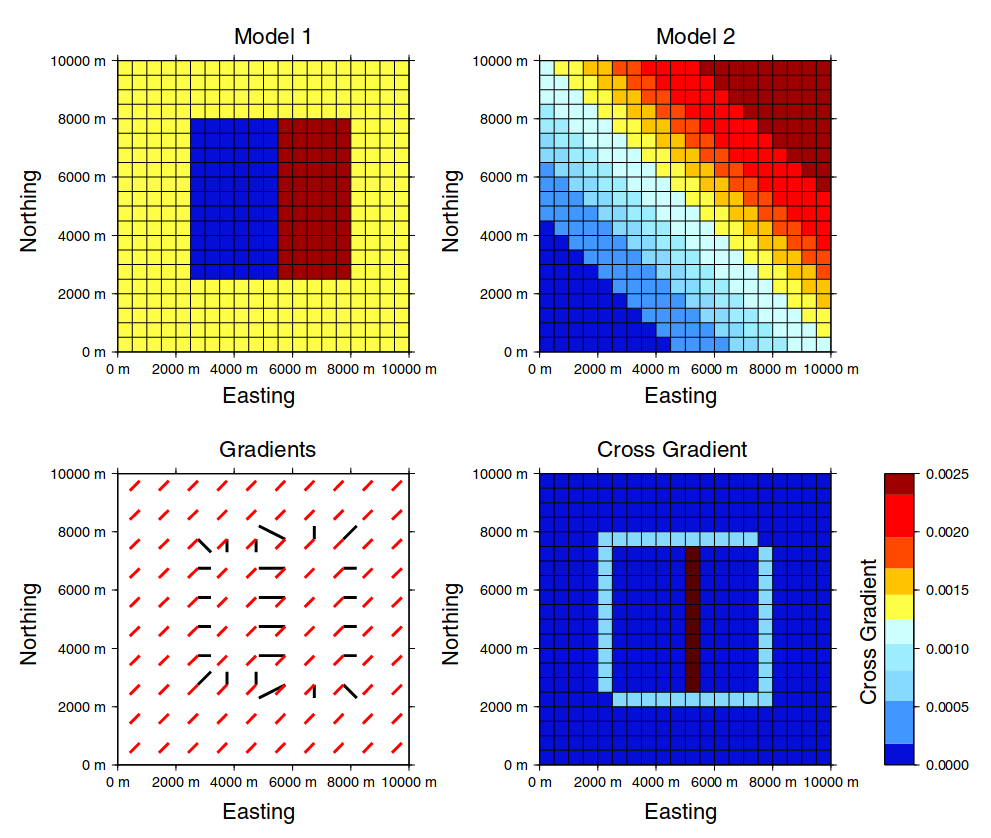
\includegraphics[width=\textwidth]{trans/trans_11.png}
    \setcounter{figure}{3}
    \caption{使用两个假设模型(模型 1,左上和模型2,右上)说明交叉梯度约束的概念草图。对于每个模型,计算并绘制空间梯度 (左下)。黑线表示模型 1的梯度,而红线表示模型 2的梯度。由此产生的交叉梯度(右下)是非零的,其中两个梯度都很显着并且指向 不同的方向}\label{trans11}

\end{figure}

在他们的案例历史中,Gallardo等(2012)反演地震速度、电阻率、密度和磁化率,因此在它们的联合反 演中包括六个交叉梯度约束,每对模型参数一个。图\ref{trans12}显示了所有数据集的单独反演和联合反演的模型参数的 所有组合的交叉梯度的大小。可以立即看出,与联合反演相比,计算单个反演结果的交叉梯度会为整个建模域中 的所有参数组合产生明显更大的值。这意味着对于大部分建模域中的单个反演,不同物理参数的变化发生在不同方向。相反,对于联合反演这些变化发生在同一方向,只有在约 2 公里深度的一个小区域显示出显着的非零交叉梯度值。加 拉多等 (2012)没有进一步讨论这种差异的可能原因,但考虑到上面教程中关于假设检验的讨论,调查 高交叉梯度值的原因将非常有趣,因为这些清楚地表明违反了相似结构的假设。检查图\ref{trans12},在观测到的磁数 据沿剖面快速变化的区域中,主要违反交叉梯度约束的发生在磁化对比度和所有其他方法之间。因此,除了 一些未知的地质原因外,这些高值也可能是由模型差异引起的,即反演网格太粗糙而无法容纳必要的变化, 或者过于乐观的数据错误。如果没有额外的信息,就不可能评估这三种效应的贡献。

\begin{figure}[H]
    \centering
    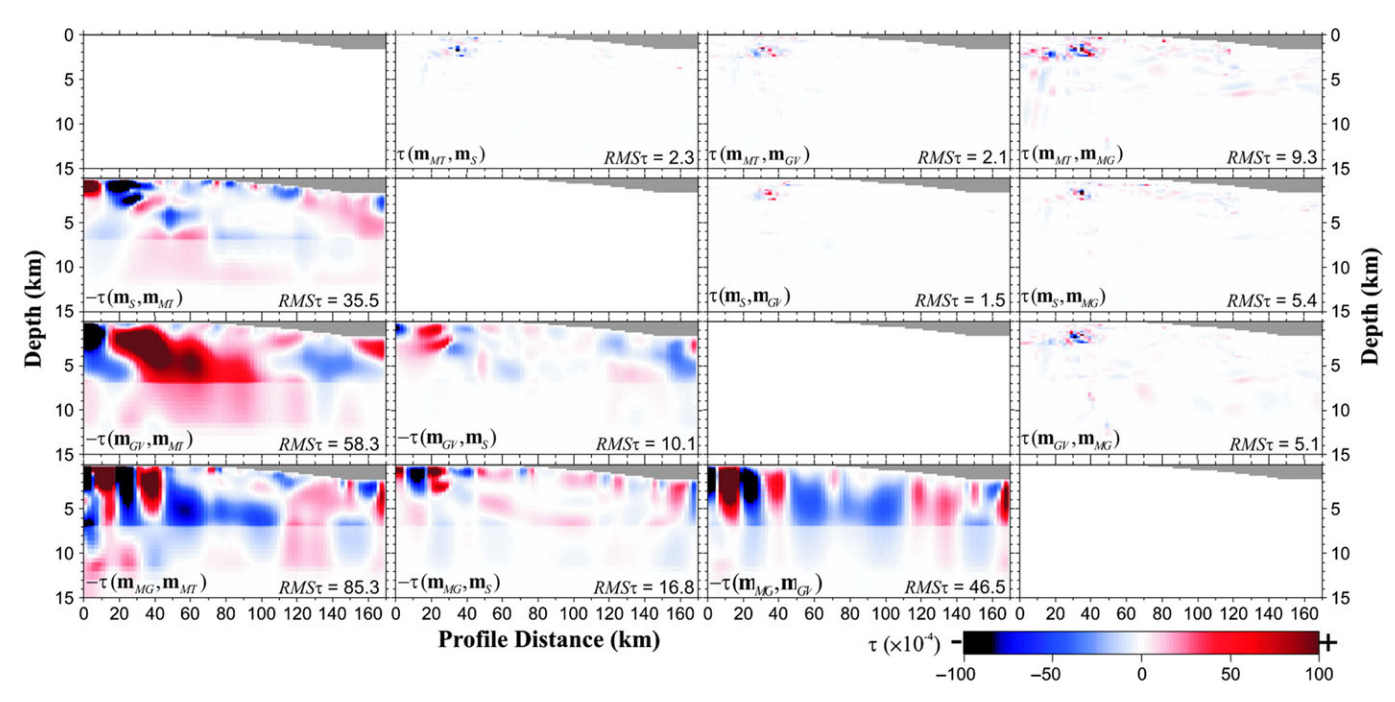
\includegraphics[width=\textwidth]{trans/trans_12.png}
    \caption{Gallardo等研究中个体反演(对角线下方)和联合反演(对角线上方)不同物理参数之间交叉梯度的大小。 (2012)}\label{trans12}
    \setcounter{figure}{2}
\end{figure}


在任何情况下,联合反演产生的模型都比单独的反演结果更相似,因此可以认为更好。多参数反演的一个问题是以易于分析的形式提炼信息。除了将不同物理特性的模型绘制成彼此相邻的传统 形式外,Gallardo等 (2012)还使用他们所谓的地理光谱图像,试图以更紧凑的形式呈现所有相关信 息。图\ref{trans13}显示了单独反演结果和联合反演的地理光谱表示。三个物理特性由不同的颜色表示,每个特性值的 变化显示为该颜色的亮度变化。第四个属性,这里是磁化,由等高线表示。结果是一个图像同时代表了所有四 个属性,其中某些颜色表示物理参数的特定组合。虽然这种表示非常紧凑并且可以很容易地识别某些岩性 单元,但一些更细微的变化会丢失,并且可以在各个地块中更容易地看到。尽管如此,这仍然是解决有效可 视化从集成反演中获得的所有信息的问题的第一步。

\begin{figure}[H]
    \centering
    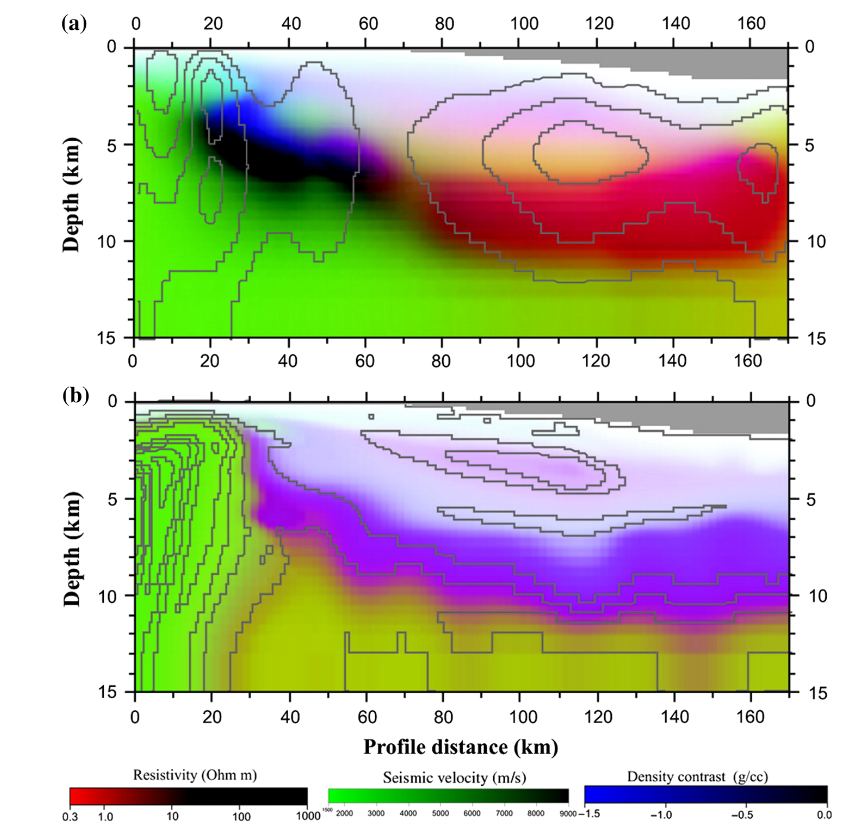
\includegraphics[width=0.9\textwidth]{trans/trans_13.png}
    \setcounter{figure}{5}
    \caption{单独反演结果(顶部)和联合反演结果的地理光谱表示(Gallardo 等, 2012 )。在这两种情况下,轮廓都显示 磁化模型}\label{trans13}
    
\end{figure}

由于灵敏度内核的减少,随着深度的增加变得更加平滑(Li和Oldenburg 1998;Streich和 Becken 2011)。由于这种灵敏度损失,正则化的影响增加,因此模型参数的变化分布更广泛,异常幅度减小。因此,与近表 面相比,深度处的交叉梯度值类似地减少了。在其他研究中也可以观察到类似的现象(参见 Moorkamp等 人, 2016a)。本宁顿等(2015)提出交叉梯度约束的归一化,以避免交叉梯度的这种自然减少,并确保深度 结构受到同样的约束。他们证明了这种方法在跨圣安德烈亚斯断层测量的合成示例和数据上的可行性。然而,到目 前为止,缺少与常规交叉梯度的仔细比较,因此,很难量化归一化对改进联合反演结果的贡献。缺乏对不同方法的 性质及其比较的系统研究是目前联合反演的普遍问题。作为一个相对年轻的领域,大多数作者都专注于开发新方法并证明这些原则上有效,只有少数研究提供了不同类型联合反演之间的比较(Moorkamp 等, 2011; Le 等, 2016)或研究了特定设置如何影响反演结果(Moorkamp 等,2016)). 随着该领域的成熟,此类研究变得越来越重要,以帮助从各种可能性中选择合适的方法。

\subsection{协同反演(Cooperative Inversion)与约束反演}

我现在将讨论一些反演案例研究,这些反演将来自其他地球物理研究的信息作为约束,但不执行联合反演。这意 味着该信息被视为对基本事实的估计,可能具有一些不确定性,但由于反演而没有反馈来修改它。正如上面教程 中所讨论的,这可能比联合反演更强烈地限制可接受模型的范围,但必须非常小心地评估约束的有效性并评估 其不确定性。

第一个约束反演案例研究(Kalscheuer 等,2015)将一系列电和电磁数据与重合地震反射剖面的约 束相结合。该研究的目的是确定博茨瓦纳Okavango三角洲的潜在地下水源。Kalscheuer 等(2015)根 据多个不同位置的分层模型联合反演音频大地电磁(AMT)、可控源AMT和瞬态电磁(TEM) 数据。地震反射剖 面用于确定到两个岩性边界的深度(1)沉积物内的边界,即所谓的POM,以及(2) 到基底的深度。在没有任何地 震约束的情况下,所有位置的三层模型都可以充分解释数据。然而,在三层反演中引入基底深度作为约束会显着 增加数据失配。向反演添加第四层允许满足约束并将数据拟合到与无约束反演相同的失配水平。这种分析类似于 上述教程和 Moorkamp 等中讨论的过程。(2010)。它再次强调了在尝试任何类型的联合反演或约束反 演之前执行单独反演的重要性,因为有必要有一个基准失配。

图\ref{trans14}显示了无约束四层反演模型(顶部)与下两个界面边界被约束匹配的反演之间的比较 从地震反射剖面解释的边界。在这种情况下,Kalscheuer 等(2015)估计这些边界深度的不确定性为10 m,但请注意,电磁数据允许与这些深度有较大偏差。约束反演的结果是所有位置的模型实际上是相同的,只有到 第一层边界的深度有一些小的波动。正如Kalscheuer 等(2015)注意这意味着电磁观测与推断的地震边界 兼容。如果我们将其视为真实地质情况的反映,则表明无约束反演的反演模型差异仅仅是数据误差到结果的映 射。

\begin{figure}[H]
    \centering
    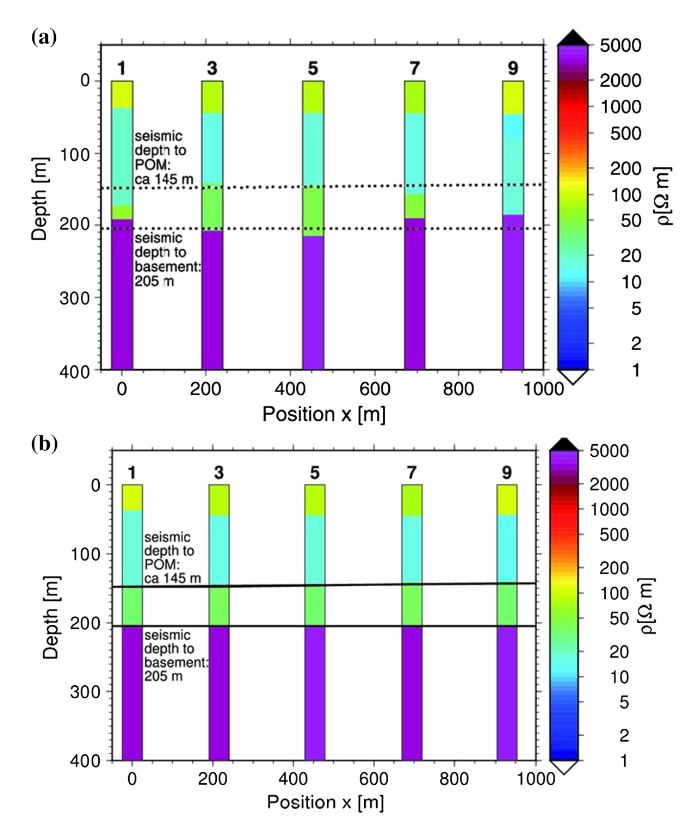
\includegraphics[width=0.9\textwidth]{trans/trans_14.png}
    \setcounter{figure}{6}
    \caption{Kalscheuer等的无约束电磁反演结果(上)与受地震数据约束的反演结果(下)对比(2015)。两组模型都将数据匹配 到可比较的失配水平。引入地震约束使模型几乎独立于位置}\label{trans14}
    
\end{figure}


在前面的例子中,地震反射数据主要显示两个强烈的水平反射,可以清楚地识别岩性边界,其余微弱的振幅 变化可归因于噪声。更一般地说,地震反射剖面,或类似的探地雷达(GPR)或偏移接收器函数图像,显示出大量 具有复杂几何形状和不同振幅的反射。尽管可以提取显着的不连续性并将信息合并到反演中(如McGary等, 2014 ),但在许多情况下并不清楚哪些反射是最重要的。在这里,半自动程序可以帮助将引导图像转换为可用于引导约束反演的形式。周等(2014)开发 了一种使用这种变换的图像引导反演方法。基于引导图像,例如 GPR剖面,计算两个量: (1) 度量张量场,用 于识别主要变化的方向和均匀性的方向,该张量的长轴与反射方向平行对齐振幅是连续的,并且(2)相似性,以识别强不连续性的位置,相似性值在主要不连续性处较低。这个过程是完全自动化的,可以应用于深 度偏移的探地雷达和地震剖面,甚至可以应用于地质剖面。为了在反演中包含张量和相似信息,有必要定义一个阈值,低于该阈值相似被认为是指示边界。

\begin{figure}[H]
    \centering
    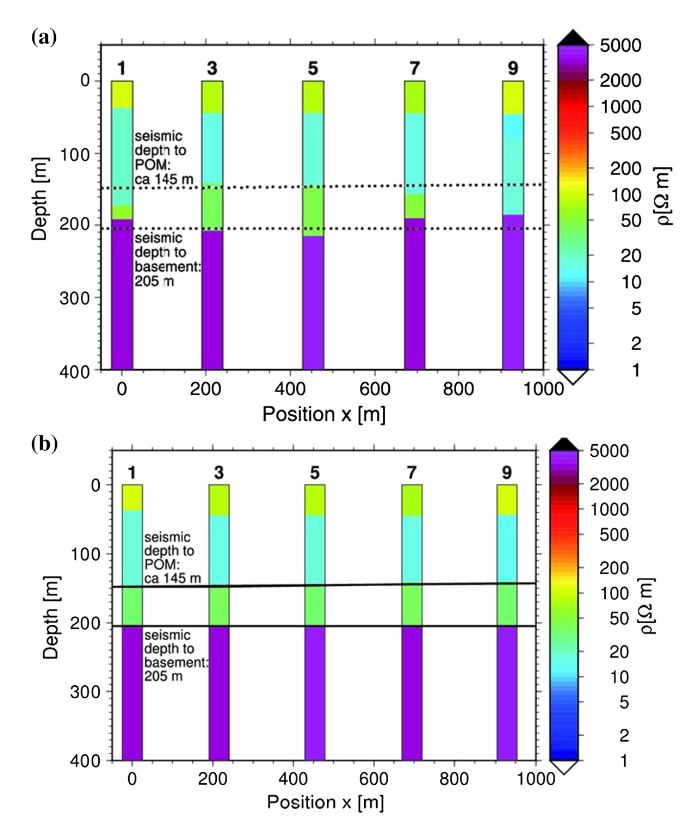
\includegraphics[width=0.9\textwidth]{trans/trans_14.png}     
    \caption{一个关于GPR引导图像的实例、计算的几个位置的度量张量场和相似度。低于用户的外观值定义的阈值用红色显示,在这些位置上,正则化被修改为沿着度量张量的长轴方向平滑,并允许沿着短轴的方向变化。在这个概念的证明中,作者使用固定的值来作为两个方向的平滑权重,但是注意这些调整这些值以反映张量轴的长度。}
    \label{trans15}
\end{figure}


定义的阈值以红色显示,在这些位置,正则化将被修改为沿度量张量的长轴方向平滑,并允许沿短轴方向变化。 在这个概念证明中,作者在这两个方向上使用固定值作为平滑权重,但请注意,可以调整这些值以反映张量轴的 长度。 在反演中引入这些约束对生成的模型有显着影响,与无约束反演相比可以看出这一点(图\ref{trans15})。正如预期的 那样,约束模型显示大部分推断边界(例如,剖面 0-15km之间)的电阻率变化更大,尽管并非所有结构都与电 阻率变化直接相关(剖面25-45km处的较低结构边界)。与无约束反演相比,数据失配仅略高,但详细查看失 配的分布并评估哪些结构对数据失配有影响以及这是否是数据中噪声的表达或由与观察不相容的约束引起的 变化。此外,应测试不同的用户定义参数、相似阈值、平滑权重的影响,并评估它们对反演结果的影响。

作为一种通用方法,图像引导反演很有吸引力,因为它可以用于仅通过适度的用户交互来引入复杂的结构信 息。 为了在反演中包含张量和相似信息,有必要定义一个阈值,低于该阈值相似被认为是指示边界。 与手动绘制的撕裂带(如,McGary 等,2014 )相比,它可用于通过使用基于相似幅度的平滑权重来允 许不同程度的结构异质性,但缺乏专家对地质意义的观察力不同的结构。然而,这是生成地球物理模型的手 动和自动程序之间的一般权衡。在专家用户手中,基于其他信息解释的正向建模和约束等手动方法可能非常强 大,但结果在很大程度上取决于用户,并且可能会因她的期望而产生偏差。大多数自动化程序(如反演算法)也需 要一些用户定义的数量,但在大多数情况下,主要结构是可比较的(如,Miensopust 等, 2013)。 图\ref{trans14}显示了基于GPR 部分的引导图像示例、计算的几个位置的度量张量场和相似度。低于用户的外观值 这两个案例研究仅展示了在反演中引入地质和地球物理信息的一些可能性。其他包括互信息(Mandolesi 和 Jones 2014),或概率反演中的地统计方法(如,Zahner等,2016、Bosch和Hansen等,2016)更详细地讨论了使用地质先验信息的理论基础。

\section{结论}

本文的教程部分展示了联合反演和约束反演方法的优缺点。明智地使用它们可以显着改善反演结果并获得更好 地反映地下的模型。然而,在复杂的自动反演算法中使用多个数据并不能减轻用户对反演模型进行批判性评估的 需要。至少,联合反演的数据失配应该与单独反演的失配匹配,但理想情况下,拟合不同数据集和所有参数的影响之间的权衡。

应探索对结果的选择。我已经描述了一些可能的方法,它们可以用作指示,在哪些情况下可以认为 集成是成功的,以及在哪些情况下必须谨慎使用。特别是当模型强烈依赖于一个或多个参数的选 择时,例如,不同数据集之间的权重或耦合约束的权重,有必要清楚地理解为什么会这样,然后才 能做出任何推论模型。

尽管存在这些困难,综合方法已经达到一定程度的成熟度,使其适用于从近地表到深层地幔的 大量区域。存在大量可以根据可用数据和先验信息进行调整的方法,上述案例研究展示了一些例 子。对于一些,例如交叉梯度耦合的联合反演,有足够的经验和系统的研究,可以清楚地了解它在哪 里可以工作,什么地方不能工作,以及应该如何使用。其他方法仍然缺乏此类信息,但随着使用的增 加,可以开发类似的策略。这对于需要大量用户定义参数和未来工作富有成果的领域的方法尤为重 要。如上所述,尽管有多种耦合方法,但仍有新发展的空间,特别是在如何将参数关系纳入联合反演 方案方面。在应用方面,包括电磁方法在内的综合方案已经在各种尺度和不同的目标上得到应用,但迄今 为止似乎缺乏针对地热勘探问题或研究地壳结构的研究。在这里可以做出具有潜在巨大影响的重大发展。
